\documentclass[11pt]{article}
\usepackage{array}
\usepackage{tabularx}
\usepackage{graphicx}
\usepackage{algorithm}
\usepackage{algorithmic}
\usepackage{pgfplotstable}
\usepackage{pgfplots}
\usepackage{filecontents}
\usepackage{amsmath}



\title{
	\textbf{IMS Assignment 2}
}

\author{Tobias Stahl \\ 10528199 \and Ioannis Giounous Aivalis \\ 10524851 }

\begin{document}

\maketitle

\section{Introduction}
This report is about Assignment 2 of the UvA course Intelligent Multimedia Systems. The goal of Assignment 2 is to implement functions to smooth images with a Gaussian filter.

\section{Exercise 1}

\subsection{Excercise 1.3 - Comparison with Built-in function}
In this exercise we observe the output of our system for an implementation of a convolution with a Gaussian filter. In that direction we first create two 1-dimentional Gaussian filter vectors, then we multiply them to get the filter matrix. Finally we convolve this matrix with the original picture to observe a blurred output picture.\\
Our implementation of those functions are located in the files \texttt{gaussian.m} and \texttt{gaussianConv.m} and the result of our tests is compared to the matlab built-in function \texttt{fspecial} for a Gaussian. Figure ~\ref{comp} shows images of the built-in function and our implementation.
\begin{figure}[h!]
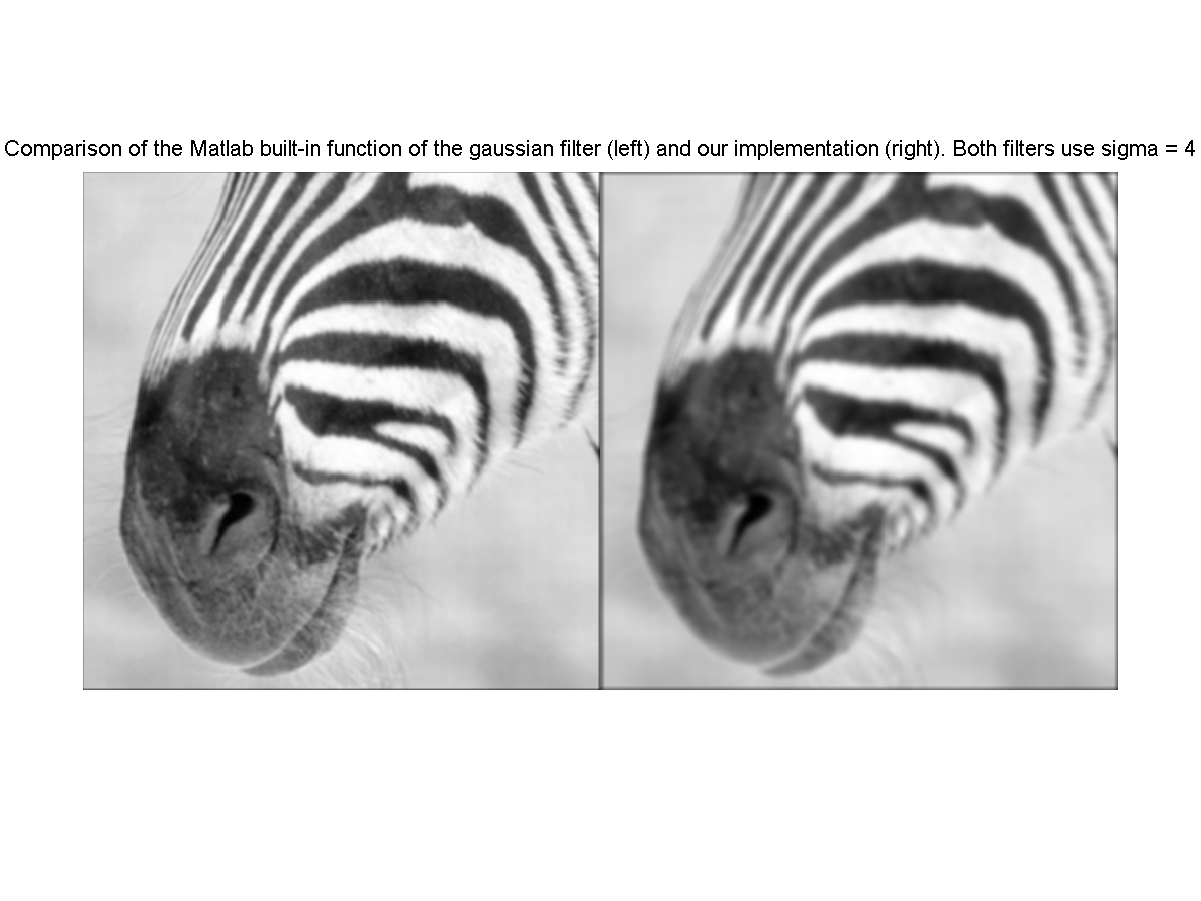
\includegraphics[scale=0.6]{comparison.png}
\caption{Comparison of matlab built-in function and our implementation }
\label{comp}
\end{figure}

\subsection{Exercise 1.5.2 - Magnitude and orientation of different $\sigma$}
In this exercise magnitude and orientation of the picture are extracted with help of functions \texttt{gaussianDer.m}, which computes the derivative of Gaussian filter G, and \texttt{gradmag.m}, which convolves the image with the derivative of the filter and returns the two images of magnitude and orientation.\\
For both the orientation and the magnitude it is clear to see, that for increasing values of $\sigma$ the smaller structures disappear and only large structures are affected by the gradient. The output of various plots are shown in Figure ~\ref{magnitude} for the magnitude and Figure ~\ref{quiv} for the orientation.
\begin{figure}[h!]
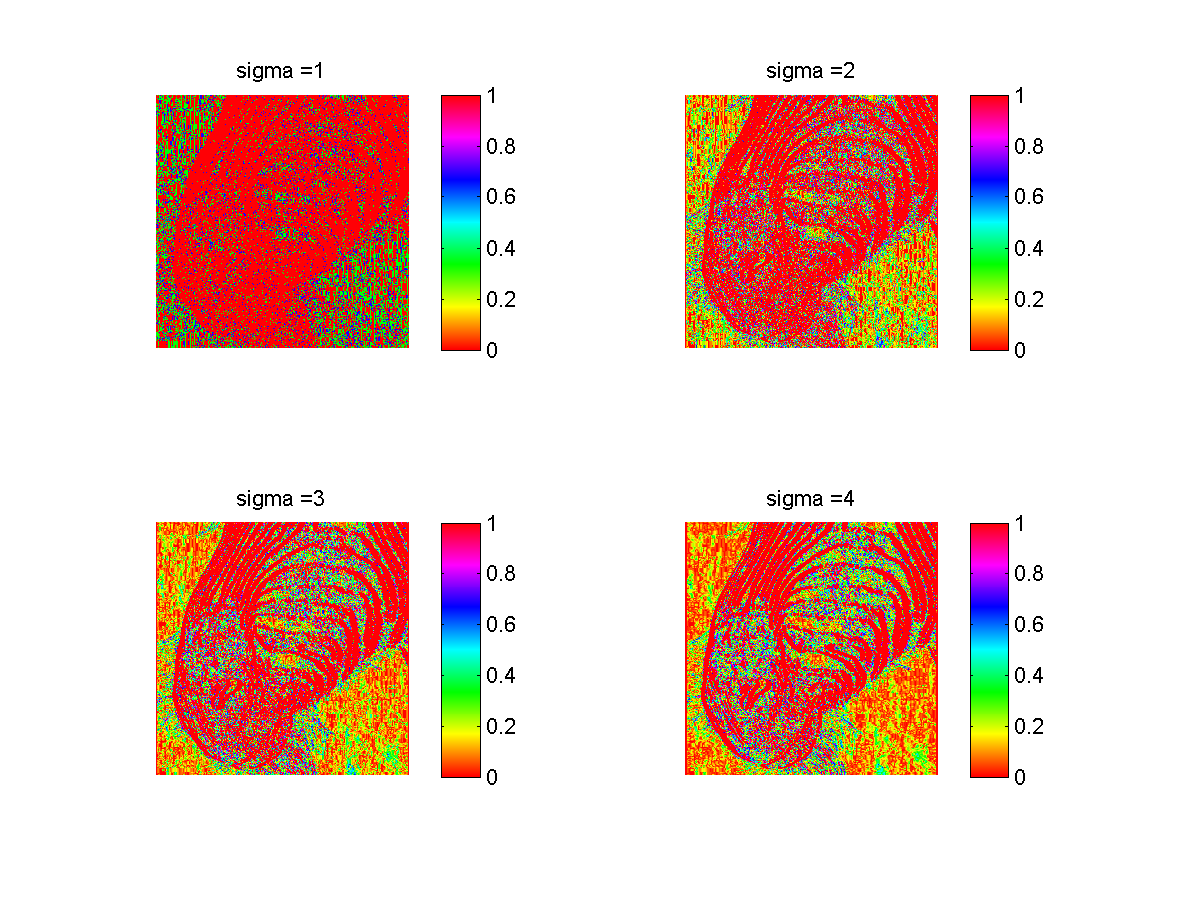
\includegraphics[scale=0.6]{magnitude.png}
\caption{Magnitude of zebra.png for $\sigma = {1,2,3,4}$}
\label{magnitude}
\end{figure}

\begin{figure}[h!]
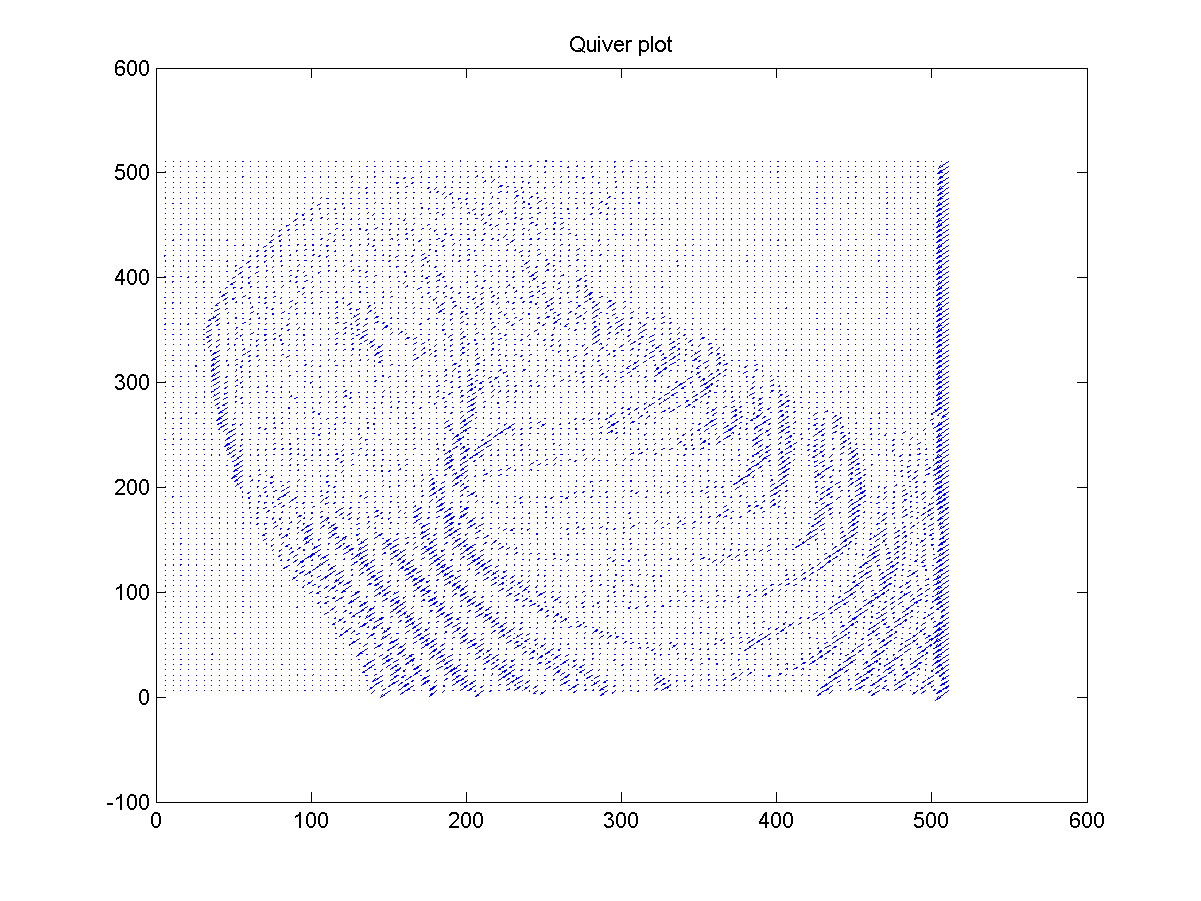
\includegraphics[scale=0.6]{quiv.png}
\caption{Orientation of zebra.png}
\label{quiv}
\end{figure}

\subsection{Exercise 1.5.3 - Thresholds}
In this section pixels of the magnitude with a value below a specific threshold are set to not appear to convert the image into a binary format. Figure ~\ref{threshold} shows the output for different thresholds and $\sigma$.

\begin{figure}[h!]
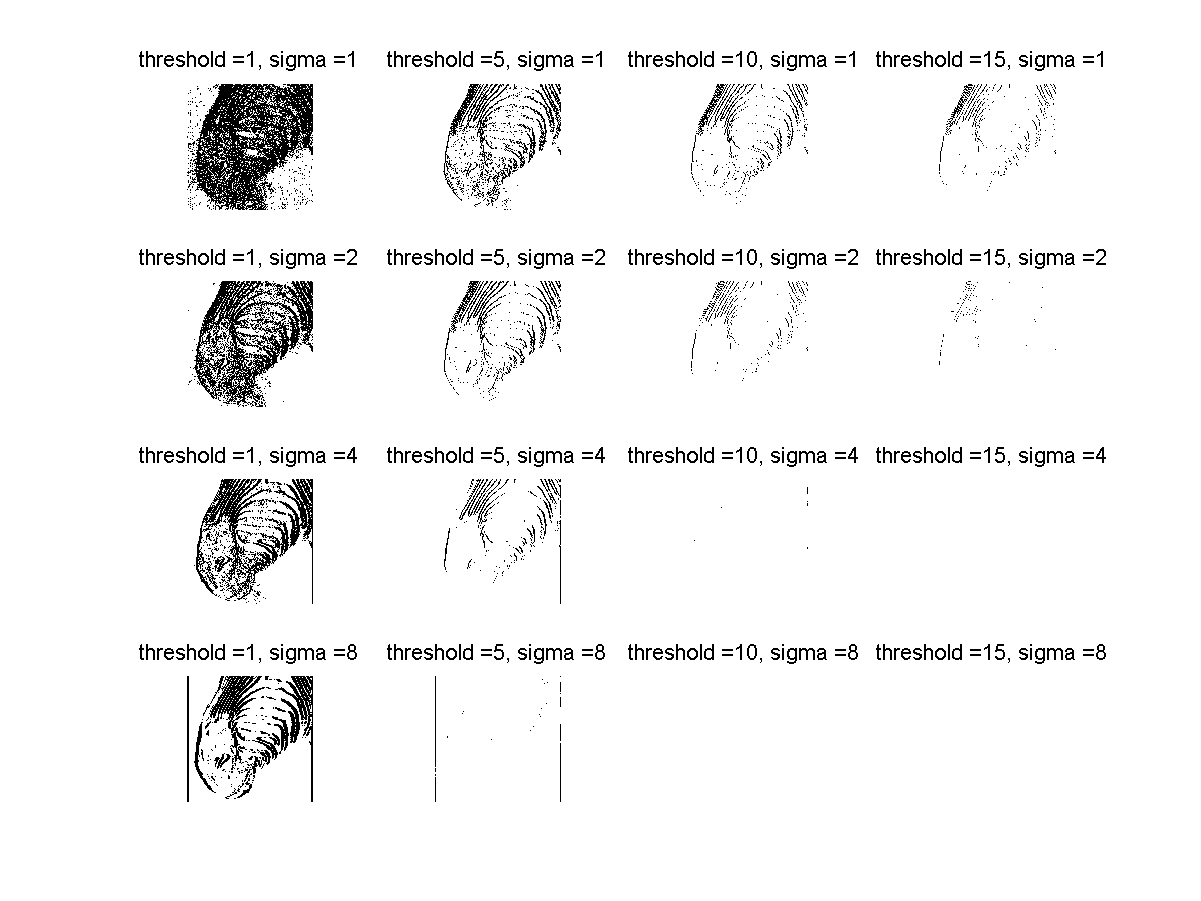
\includegraphics[scale=0.6]{threshold.png}
\caption{Magnitudes after threshold filter}
\label{threshold}
\end{figure}

\subsection{Exercise 1.5.5 - Impulse}
For this exercise we first create an impulse picture initialized with zeros (black) and set the center pixel color to white. Next we create various Gaussian filters with different orientations (x-axis, y-axis etc.) and convolve with the impulse picture.\\
The result image is suppose to display the filter. Figure ~\ref{impulse} shows the result images of this exercise.

\begin{figure}[h!]
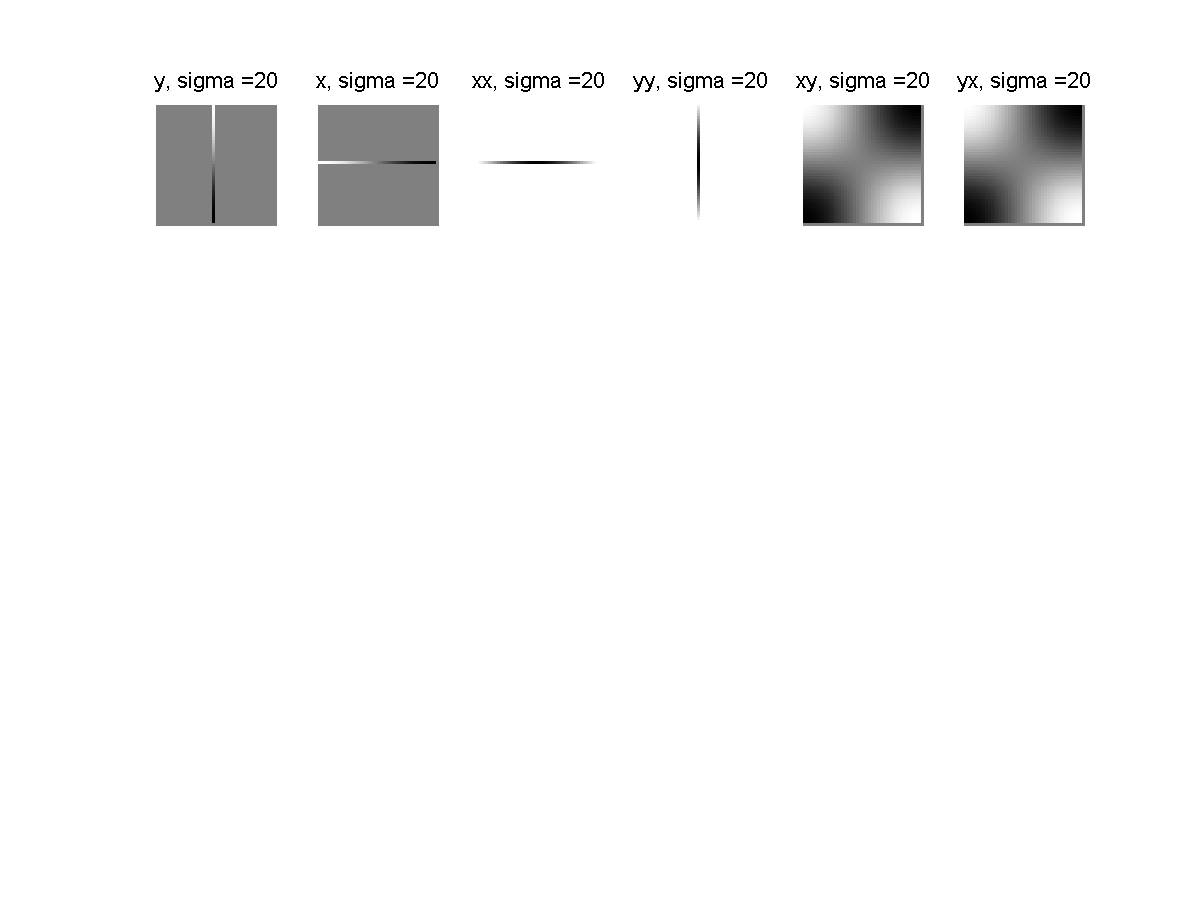
\includegraphics[scale=0.6]{impulse.png}
\caption{Filter on impulse image}
\label{impulse}
\end{figure}

\section{Conclusion}
In this assignment the functions to create a Gaussian filter and its derivatives, and to convolve those with any image were implemented and tested with different exercises. 




\end{document}